\def\bs{$\backslash$}
\chapter{راهنماهای نصب}\label{c1}
\section{نصب تک‌لایو}
به دو طریق می‌توانید تک‌لایو ۲۰۱۱ را نصب کنید.
\begin{enumerate}
\item
با استفاده از منبع برنامه که ممکن است با دی‌وی‌دی یا فلش به دست شما رسیده باشد، اما دانشجویان دانشگاه فردوسی می‌توانند نسخه نصبی را از اول مهر ماه ۹۰ آن را از مسیر \lr{ftp://}، در داخل شبکه دانشگاه نیز دانلود کنند.
\item
با استفاده از اینترنت
\end{enumerate}
\subsection{نصب از روی منبع}
در این روش شما باید سه مرحله زیر را انجام دهید.
\begin{enumerate}[a.]
\item
مطابق شکل زیر روی \lr{0\_texlive\_2011.exe} کلیک کنید و در پنجره‌ای که باز می‌شود ok را کلیک کنید تا فایل فشرده استخراج شود.(توجه داشته باشید که برای انتقال فقط از همان نسخه فشرده استفاده کنید، چون در غیر این‌صورت باید زمان زیادی صرف کنید)\\
در ادامه برای شروع فرآیند نصب بایست به داخل پوشه \lr{texlive} بروید و سپس فایل \lr{install-tl.bat} را اجرا کنید، در این زمان بایست طی حداکثر چند دقیقه یک پنجره سیاه‌رنگ باز شود و پس از آن صفحه خوش‌آمدگویی تک‌لایو ۲۰۱۱ که به شکل زیر است.

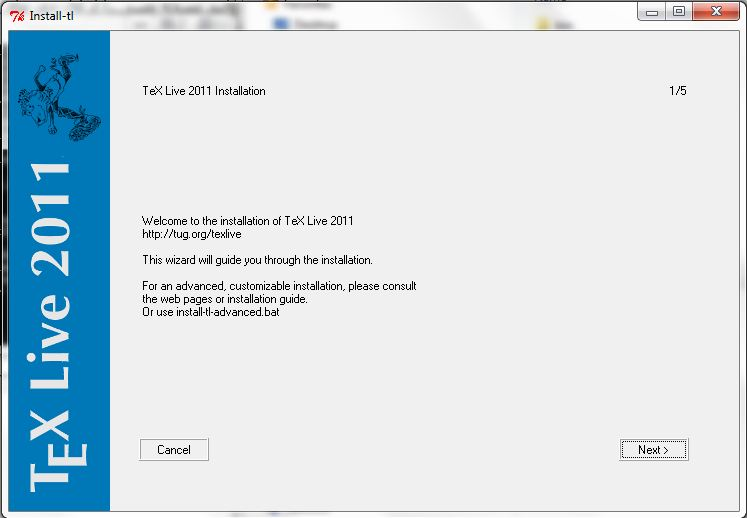
\includegraphics[scale=.5]{fig/welcome}

در ادامه راه شما فقط باید بدون تغییر هیچ چیز فقط به مراحل بعدی نصب بروید(عملا در سه پنجره اولی که باز می‌شوند فقط کافی‌ست \lr{next} و در پنجره چهارم هم \lr{install} را باید کلیک کنید.\\
بعد از انجام این مراحل دو صفحه یکی سیاه رنگ و دیگری آبی‌-خاکستری دارید که بسته‌های در حال نصب را نمایش می‌دهند. ۳۰ تا ۴۵ دقیقه که بگذرد دیگه باید نصب بسته‌ها تموم بشه و زیر صفحه دکمه \lr{finish} ظاهر بشه، روی اون کلیک کنید. در این‌جا مرحله اول تمام می‌شود و تک‌لایو به طور کامل نصب شده است.(نصب تک‌لایو در حقیقت اصلی‌ترین مرحله است و روح کار است در مراحل بعدی شما فقط ورودی برای استفاده از آن خواهید ساخت)
\item
در این مرحله باید ادیتور \lr{Texmaker} را نصب کنید(با نصب ادیتور شما می‌توانید از تک‌لایو نصب شده استفاده کنید، به این صورت که فایل را در ادیتور باز کرده و با اجرای آن ادیتور با اتصال به تک‌لایو تبدیل فایل متنی کد را به فایل پی‌دی‌اف ممکن می‌سازد) برای انجام این کار کافی‌ست شما به پوشه \lr{1\_Texmaker} بروید و تنها فایل درون آن به نام 
\lr{Texmaker\_BiDi-0.6.10\_STATIC\_installer.exe} را اجرا کنید و بدون هیچ تغییری فقط موافقت‌تان با نصب برنامه را اعلام کنید و تا آخر ادامه دهید.(تا این‌جا ادیتور هم نصب شد)
\item
در مرحله آخر فقط باید فونت‌های لازم را از  پوشه \lr{2\_FarsiFonts} به پوشه \lr{C:\bs Windows\bs Fonts} کپی کنید.
\end{enumerate}
خسته نباشید، شما به پایان نصب رسیدید. حال کافی‌ست یک فایل آماده با توسعه‌ی \lr{tex} را باز کرده و با زدن فلش آبی کنار \lr{QuickBuild} فایل را اجرا کرده و بعد از اتمام اجرا با زدن فلش آبی کنار \lr{ViewPDF} خروجی را مشاهده کنید. اما این فایل نمونه را که یک نمونه رساله برای دانشگاه فردوسی مشهد است را ما در پوشه‌ای به نام \lr{FThesis} آماده کرده‌ایم که شما بایست فایل \lr{main.tex} را از داخل آن انتخاب و در ادیتور \lr{Texmaker} اجرا کنید.
\subsection{نصب مستقیم با اینترنت}
در این روش شما به صورت مستقیم وارد مراحل نصب می‌شوید، بدیهی است که چنانچه در طول فرآیند نصب اتصال شما به اینترنت قطع شود دوباره باید نصب را از سر بگیرید.\\
این روش به زودی تشریح می‌شود.
\subsection{نصب غیرمستقیم با اینترنت}
در این روش شما ابتدا فایل‌های نصب را از اینترنت تهیه کرده و بعد به نصب از روی آن خواهید پرداخت. در این روش لزومی ندارد که حتما در یک بار اتصال تمام دریافت فایل انجام شود.\\
این روش به زودی تشریح می‌شود.
%\section{تغییراتی که بایست برای استفاده از بیمر به صورت فارسی داده شود}
%بیمر بسته‌ای برای طراحی اسلاید است که با زی‌پرشین سازگار نیست و با بسته جدید لواپرشین که برای رفع نواقص زی‌پرشین(از جمله عدم پشتیبانی همین بسته کارامد بیمر) اقدام به تولید آن شده است، سازگار است.
%
%برای نصب شما بایست  مرحله زیر را انجام دهید.
%\begin{enumerate}
%\item
%نصب لواپرشین.\\
%به دایرکتوری \lr{C:\bs texlive\bs 2011\bs texmf-dist\bs tex\bs lualatex} بروید چنانچه پوشه‌ای به نام \lr{luapersian} دیدید و نیز فایلی به نام \lr{luapersian.sty} را درون آن یافتید بدانید که این بسته نصب شده در غیر این صورت بایست خودتان پوشه \lr{luapersian} را از پوشه \lr{beamer} همراه با این راهنما برداشته و در مسیری که در بالا گفتیم قرار دهید(\lr{C:\bs texlive\bs 2011\bs texmf-dist\bs tex\bs lualatex}) تا این جا نصب لواپرشین به اتمام رسیده و برای تست آن بایست حتما یک‌بار سیستم را ریست کنید(البته راه ساده‌تری هم برای اهل فن هست).
%\item
%در این مرحله شما باید فایلی به نام \lr{beamerbasetheorems.sty} را که برای تولید محیط‌های شماره‌دار فارسی دست‌کاری شده و در پوشه \lr{beamer} همراه با این راهنماست را با فایلی که با همین نام و در مسیر \lr{C:\bs texlive\bs 2011\bs texmf-dist\bs tex\bs latex\bs beamer} قرار دارد تعویض کنید(گفتیم تعویص تا اگر خواستید از بیمر در متون انگلیسی استفاده کنید دوباره با همین تعویض امکانش مهیا باشد، چون در حقیقت فایل \lr{beamerbasetheorems.sty} پیش‌فرض برای محیط لاتین و فایل \lr{beamerbasetheorems.sty} دست‌کاری شده توسط ما برای محیط فارسی مناسب است.)
%\item
%تنها کاری که مانده این است که تک‌میکر را برای اجرای لواپرشین آماده کنید، به این منظور به سراغ \lr{TeXmaker} رفته و از منوی \lr{Options} یا معادل فارسی آن \lr{Configure Texmaker} یا معادل فارسی آن را برگزینید. در پنجره‌ای که باز می‌شود و در سمت چپ آن بر روی شکلک \lr{Commands} کلیک کنید و در خط اول مقابل \lr{LaTeX}، عبارت \hbox{\lr{lualatex -interaction=nonstopmode -synctex=-1\; \%.tex}} را به طور دقیق بنویسد حال برای اجرا فایل امتحانی به سراغ فایل \lr{main} در پوشه \lr{sample}، در پوشه \lr{beamer} همراه این راهنما بروید. آن را با \lr{TeXmaker} باز کنید و با تنظیم اجرا قرار دادن نوار اجرا بر روی \lr{LaTeX} فلش آبی کنار آن را برای اجرا و فلش آبی بعد از آن را برای دیدن خروجی کلیک کنید.
%\begin{center}
%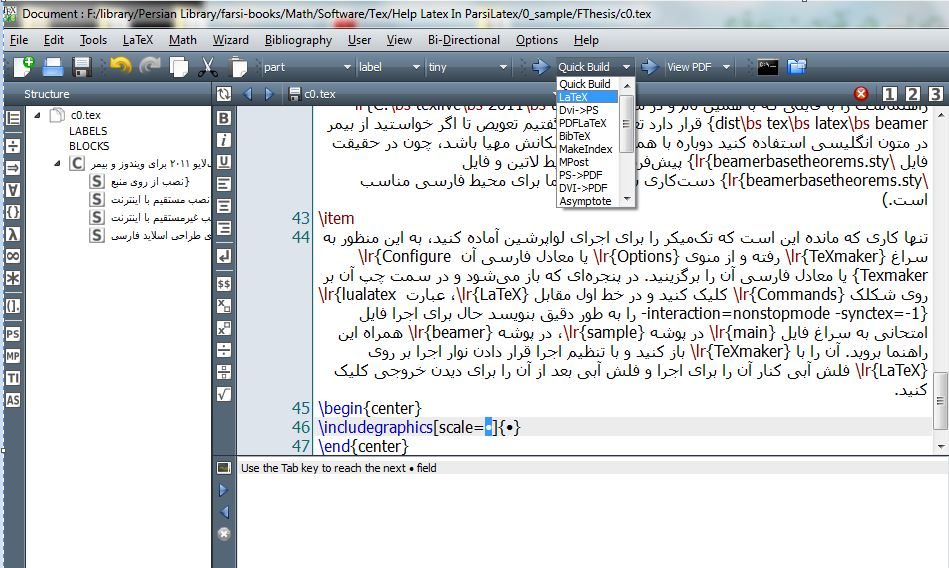
\includegraphics[scale=.3]{fig/beamer}
%\end{center}
%\end{enumerate}
\section{راه‌اندازی xindy برای تولید نمایه}
برای ایجاد نمایه شما لازم است ۴ فایل را برای اضافه کردن زبان فارسی اضافه کنید. این فایل‌ها در پوشه‌ای به نام \lr{persian} در پوشه \lr{TeX\;Pakage} قرار دارند، آن‌ها را در مسیر \lr{C:\bs texlive\bs 2011\bs texmf\bs xindy\bs modules\bs lang\bs} کپی کنید و بعد \lr{Command\;Prompt} را باز کنید و دستور \lr{texhash} را بزنید و مقداری تامل کنید تا عبارت \lr{done} را ببینید. حال اگر \lr{bidiTeXmaker} نسخه 3.1.0-3 را طبق دستورات بالا نصب کردید به سراغ منوی \lr{Tools} بروید و دستور \lr{Xindy Make Index} را برای تولید فایل مربوط به نمایه اجرا کنید و سپس فایل را اجرا کنید و خروجی را ببینید.